\hsection{Relationship Attributes}%
%
\begin{figure}%
\centering%
%
\subfloat[][%
A reproduction of \cref{fig:erdPerson2} from back in \dref{sec:conceptual:relationships}, which was created using \yEd.%
\label{fig:erdPerson1B}%
]{\includegraphics[width=0.9\linewidth]{\figErdPersonII}}%
%
\floatRowSep%
%
\subfloat[][%
A transformation of \cref{fig:erdPerson1B} to a logical model using \pgmodeler.%
\label{fig:logicalPerson2}%
]{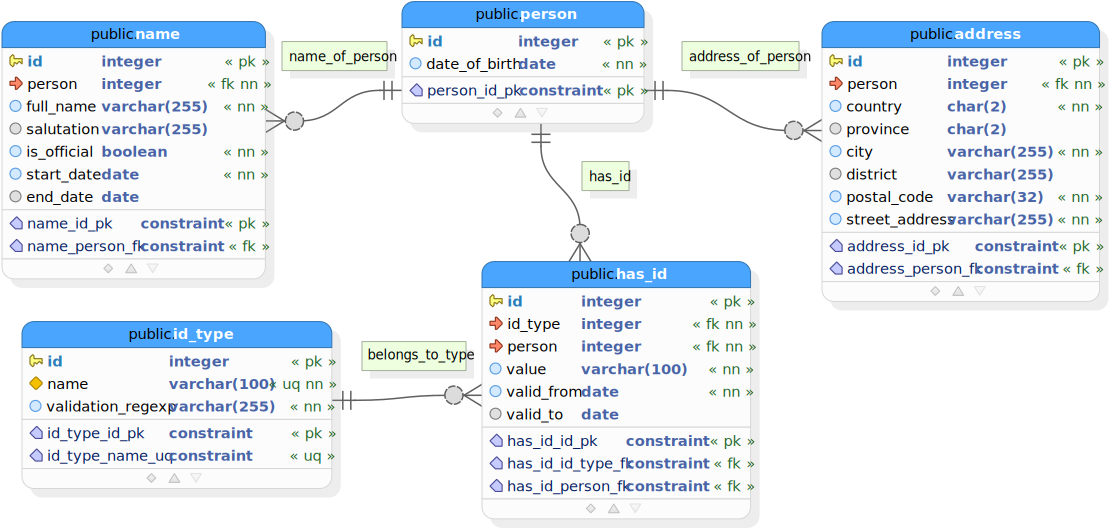
\includegraphics[width=0.9\linewidth]{\currentDir/logicalPerson2}}%
%
\caption{The representation of relationship attributes as table for the relationship.}%
\label{fig:logicalPerson2X}%
\end{figure}%
%
Relationships in conceptual models may have attributes, as stated in \cref{def:relationshipAttribute}.
Of course, since relationships do not exist as distinct objects in the relational data model, we must find another way to express these attributes.
Since only relations exist in the relational model and such relations become tables in a \db, the attributes of relationships also become table columns.

It will depend on the relationship pattern where we put them.
To try this concept out, let us go back to an even earlier example of the \emph{Person} entity:
to \cref{fig:erdPerson2} from back in \dref{sec:conceptual:relationships}.
We created this figure using \yEd\ and reprint it in \cref{fig:erdPerson1B}.
As you can see, in this figure, there is a relationship \emph{has~ID} that connects the \emph{Person} entities with the entity type~\emph{ID~Type}.

In the model, we did not annotate the relationships with cardinalities, because that was before we got to that topic.
However, it is rather clear that this would either be a \crowsFoot{\emph{Person}}{OM}{\emph{ID Type}}{OM} or a \crowsFoot{\emph{Person}}{MM}{\emph{ID Type}}{OM} relationship.
We can store arbitrarily many forms of ID for each person and each form of ID may be used by arbitrarily many people.
Since we went the hard way in the last section and modeled a relationship with the \emph{mandatory many} pattern, we this time go easy and choose \crowsFoot{\emph{Person}}{OM}{\emph{ID Type}}{OM}.
In other words, we follow the pattern \crowsFoot{O}{OM}{P}{OM} discussed in \dref{sec:rm:op}.

For this pattern, we need an additional table.
We follow exactly the same method as back in \cref{sec:rm:op}, except that we use different table and column names.
We also use \pgmodeler\ for the sake of convenience~(and because it allows me to create nice \pglspl{ERD}\dots).
We call the additional table \sqlil{has_id} to properly reflect the conceptual model.
The relationship attributes will therefore become columns of this table.
This is illustrated in \cref{fig:logicalPerson2}.

Notice how we again gain another perspective on how we modeled relationships:
In \cref{sec:rm:op}, we implement an \crowsFoot{O}{OM}{P}{OM} relationship in \sql.
We did so using the additional table~\sqlil{relate_o_and_p}.
Another perspective would be that we actually implemented two relationships:
\crowsFoot{\sqlil{o}}{M1}{\sqlil{relate_o_and_p}}{OM} and \crowsFoot{\sqlil{p}}{M1}{\sqlil{relate_o_and_p}}{OM}.
Each row in table~\sqlil{relate_o_and_p} must be related to one row in table~\sqlil{o} and also to one row in table~\sqlil{p}.
Each row in table~\sqlil{o} can be related to arbitrarily many rows in table~\sqlil{relate_o_and_p}.
Each row in table~\sqlil{p} can be related to arbitrarily many rows in table~\sqlil{relate_o_and_p}.
Indeed, that forms a \crowsFoot{O}{OM}{P}{OM} relationship.

Also, when implementing the full conceptual model given in \cref{fig:erdPerson1B}, we again encounter multi-valued attributes:~\emph{Name} and \emph{Address}.
As we already learned before, these go into additional tables, which we call \sqlil{name} and \sqlil{address}, respectively.
For these, we again use the proper foreign key \sqlilIdx{REFERENCES} constraints.

\gitSQL{\databasesCodeRepo}{teachingManagement/logical/person_database_2/generated_sql/01_person_database_database_2001.sql}{person_2:01_person_database_database_2001}{The generated script to create the \sqlil{person_database}~\db.}%
\gitExec{\databasesCodeRepo}{.}{_scripts_/postgres.sh teachingManagement/logical/person_database_2/generated_sql 01_person_database_database_2001.sql}%
%
\gitSQL{\databasesCodeRepo}{teachingManagement/logical/person_database_2/generated_sql/03_public_person_table_5071.sql}{person_2:03_public_person_table_5071}{The generated \sql\ script to create the table~\sqlil{person}.}%
\gitExec{\databasesCodeRepo}{.}{_scripts_/postgres.sh teachingManagement/logical/person_database_2/generated_sql 03_public_person_table_5071.sql person_database}%
%
\gitSQL{\databasesCodeRepo}{teachingManagement/logical/person_database_2/generated_sql/04_public_name_table_5075.sql}{person_2:04_public_name_table_5075}{The generated \sql\ script to create the table~\sqlil{name}.}%
\gitExec{\databasesCodeRepo}{.}{_scripts_/postgres.sh teachingManagement/logical/person_database_2/generated_sql 04_public_name_table_5075.sql person_database}%
%
\gitSQL{\databasesCodeRepo}{teachingManagement/logical/person_database_2/generated_sql/05_public_address_table_5084.sql}{person_2:05_public_address_table_5084}{The generated \sql\ script to create the table~\sqlil{address}.}%
\gitExec{\databasesCodeRepo}{.}{_scripts_/postgres.sh teachingManagement/logical/person_database_2/generated_sql 05_public_address_table_5084.sql person_database}%
%
\gitSQL{\databasesCodeRepo}{teachingManagement/logical/person_database_2/generated_sql/06_public_id_type_table_5094.sql}{person_2:06_public_id_type_table_5094}{The generated \sql\ script to create the table~\sqlil{id_type}.}%
\gitExec{\databasesCodeRepo}{.}{_scripts_/postgres.sh teachingManagement/logical/person_database_2/generated_sql 06_public_id_type_table_5094.sql person_database}%
%
\gitSQL{\databasesCodeRepo}{teachingManagement/logical/person_database_2/generated_sql/07_public_has_id_table_5100.sql}{person_2:07_public_has_id_table_5100}{The generated \sql\ script to create the table~\sqlil{has_id}.}%
\gitExec{\databasesCodeRepo}{.}{_scripts_/postgres.sh teachingManagement/logical/person_database_2/generated_sql 07_public_has_id_table_5100.sql person_database}%
%
\gitSQL{\databasesCodeRepo}{teachingManagement/logical/person_database_2/generated_sql/08_public_name_name_person_fk_constraint_5108.sql}{person_2:08_public_name_name_person_fk_constraint_5108}{The generated \sql\ script to create the foreign key constraint ensuring that each row in table~\sqlil{name} is associated with one row in table~\sqlil{person}.}%
\gitExec{\databasesCodeRepo}{.}{_scripts_/postgres.sh teachingManagement/logical/person_database_2/generated_sql 08_public_name_name_person_fk_constraint_5108.sql person_database}%
%
\gitSQL{\databasesCodeRepo}{teachingManagement/logical/person_database_2/generated_sql/09_public_address_address_person_fk_constraint_5109.sql}{person_2:09_public_address_address_person_fk_constraint_5109}{The generated \sql\ script to create the foreign key constraint ensuring that each row in table~\sqlil{address} is associated with one row in table~\sqlil{person}.}%
\gitExec{\databasesCodeRepo}{.}{_scripts_/postgres.sh teachingManagement/logical/person_database_2/generated_sql 09_public_address_address_person_fk_constraint_5109.sql person_database}%
%
\gitSQL{\databasesCodeRepo}{teachingManagement/logical/person_database_2/generated_sql/10_public_has_id_has_id_id_type_fk_constraint_5110.sql}{person_2:10_public_has_id_has_id_id_type_fk_constraint_5110}{The generated \sql\ script to create the foreign key constraint ensuring that each row in table~\sqlil{has_id} is associated with one row in table~\sqlil{id_type}.}%
\gitExec{\databasesCodeRepo}{.}{_scripts_/postgres.sh teachingManagement/logical/person_database_2/generated_sql 10_public_has_id_has_id_id_type_fk_constraint_5110.sql person_database}%
%
\gitSQL{\databasesCodeRepo}{teachingManagement/logical/person_database_2/generated_sql/11_public_has_id_has_id_person_fk_constraint_5111.sql}{person_2:11_public_has_id_has_id_person_fk_constraint_5111}{The generated \sql\ script to create the foreign key constraint ensuring that each row in table~\sqlil{has_id} is associated with one row in table~\sqlil{person}.}%
\gitExec{\databasesCodeRepo}{.}{_scripts_/postgres.sh teachingManagement/logical/person_database_2/generated_sql 11_public_has_id_has_id_person_fk_constraint_5111.sql person_database}%
%
\gitSQLAndOutput{\databasesCodeRepo}{teachingManagement/logical/person_database_2}{insert.sql}{person_database}{}{}{postgres.sh}{person_database_2:insert}{%
Inserting into the tables in the \sqlil{person_database}.}%
%
\gitSQLAndOutput{\databasesCodeRepo}{teachingManagement/logical/person_database_2}{select.sql}{person_database}{}{}{postgres.sh}{person_database_2:select}{%
Selecting data from the tables in the \sqlil{person_database}.}%

We can export the logical model created with \pgmodeler\ and we get \cref{lst:person_2:01_person_database_database_2001,lst:person_2:03_public_person_table_5071,lst:person_2:04_public_name_table_5075,lst:person_2:05_public_address_table_5084,lst:person_2:06_public_id_type_table_5094,lst:person_2:07_public_has_id_table_5100,lst:person_2:08_public_name_name_person_fk_constraint_5108,lst:person_2:09_public_address_address_person_fk_constraint_5109,lst:person_2:10_public_has_id_has_id_id_type_fk_constraint_5110,lst:person_2:11_public_has_id_has_id_person_fk_constraint_5111}.
\Cref{lst:person_2:01_person_database_database_2001} creates the \db\ \sqlil{person_database}.
The table \sqlil{person} is created in \cref{lst:person_2:03_public_person_table_5071}, with a surrogate primary key and a field \sqlil{date_of_birth} for the \pgls{dateOfBirth}.

In \cref{lst:person_2:04_public_name_table_5075}, the table \sqlil{name} is created for the multi-valued composite attribute \emph{Name}.
Each row in table~\sqlil{name} will store a foreign key~\sqlil{person} that is linked to a row in table~\sqlil{person} using a \sqlilIdx{REFERENCES} constraint, which is added later in \cref{lst:person_2:08_public_name_name_person_fk_constraint_5108}.
Apart from that, we added a small gimmick for your enjoyment:
The column \sqlil{start_date} is created \sqlil{NOT NULL DEFAULT CURRENT_DATE}.
This means that, for each row in table~\sqlil{name}, we must \emph{store} a proper start date as per the~\sqlilIdx{NOT NULL}.
However, if we do not \emph{provide} such a date when the row is created, a \sqlilIdx{DEFAULT} value is stored instead.
This \sqlilIdx{DEFAULT} is \sqlil{CURRENT_DATE}\sqlIdx{CURRENT\_DATE}, which, as the name implies, will be the date at the very moment we enter the row into the \db~\cite{PGDG:PD:DTFAO}.
Similar functions are \sqlil{CURRENT_TIME}\sqlIdx{CURRENT\_TIME} and, most importantly, \sqlil{CURRENT_TIMESTAMP}\sqlIdx{CURRENT\_TIMESTAMP}~\cite{PGDG:PD:DTFAO}, which is often used for \pgls{timestamping}.

But back to the topic at hand.
\Cref{lst:person_2:05_public_address_table_5084} creates the table~\sqlil{address}.
There is nothing special about this table.
Its foreign key~\sqlil{person} is related to the table~\sqlil{person} using the \sqlilIdx{REFERENCES} constraint given in \cref{lst:person_2:09_public_address_address_person_fk_constraint_5109}.
\Cref{lst:person_2:06_public_id_type_table_5094} creates the table~\sqlil{id_type} in pretty much the same shape and form already used in the previous section in \cref{lst:person_1:04_public_id_type_table_5072}.
The table~\sqlil{has_id} is created in \cref{lst:person_2:07_public_has_id_table_5100}.
It follows the same design as table~\sqlil{personal_id} from the previous section, which was given in \cref{lst:person_1:05_public_personal_id_table_5078}.
The corresponding foreign key constraints linking its rows to tables~\sqlil{id_type} and~\sqlil{person} are created using \cref{lst:person_2:11_public_has_id_has_id_person_fk_constraint_5111,lst:person_2:10_public_has_id_has_id_id_type_fk_constraint_5110}, respectively.
With this, we have constructed the \sqlil{person_database}.

We fill the \db\ with data in \cref{lst:person_database_2:insert}.
In \cref{lst:person_database_2:select}, we use a query that combines data from several tables using \sqlilIdx{INNER JOIN} statements and then concatenates the data to single text strings per result row.%
%
\FloatBarrier%
\endhsection%
%
